%
\documentclass[12pt,notitlepage]{article}
\usepackage{amssymb}
\usepackage{amsmath}
\usepackage{graphicx}
\usepackage{epstopdf}
\usepackage{pdflscape}
\usepackage[pdftex,dvipsnames]{xcolor}  
\setlength{\marginparwidth}{2cm}
\usepackage[colorinlistoftodos,prependcaption,textsize=small]{todonotes}
\usepackage{xargs}
\usepackage{tabularx}
\usepackage{longtable}
\usepackage{array}
\usepackage{dsfont}
\usepackage{float}
\usepackage{booktabs}
\usepackage{tikz}
\usepackage{marvosym}
\usepackage{multirow}
\usepackage{pdflscape}
\usepackage[hyphens]{url}
\usepackage{setspace}
\usepackage{epigraph}
\usepackage{bm}
\usepackage{textcomp}
\usepackage{diagbox}
\usepackage{bbm}
\usepackage{verbatim}
\usepackage[framemethod=tikz]{mdframed}
\usepackage{subcaption}
\usepackage{caption}
\usepackage{lipsum}
\usepackage{mathtools}
\usepackage{scalerel}
\usepackage{stackengine}
\usepackage{amsthm}
\usepackage{epsfig}
\usepackage[
backend=bibtex,
style=authoryear-comp,
sorting=ynt
]{biblatex}
\usepackage[colorlinks,allcolors=blue]{hyperref}
\usepackage[shortlabels]{enumitem}
\usepackage{subfiles} % Best loaded last in the preamble


\setlength{\epigraphrule}{0pt}
\renewcommand{\baselinestretch}{1.25}

\setcounter{MaxMatrixCols}{10}

\newcolumntype{L}[1]{>{\raggedright\let\newline\\\arraybackslash\hspace{0pt}}m{#1}}
\newcolumntype{C}[1]{>{\centering\let\newline\\\arraybackslash\hspace{0pt}}m{#1}}



\newcommand{\I}{\mathbb{I}}
\newcommand{\E}{\mathbb{E}}
\newcommand{\Ll}{\mathrm{L}}
\newcommand{\R}{\mathbb{R}}
\renewcommand{\L}{\mathbb{L}}
\newcommand{\Var}{\mathrm{Var}}
\newcommand{\Cov}{\mathrm{Cov}}
\newcommand{\Corr}{\mathrm{Corr}}
\newcommand{\Prob}{\mathbb{P}}
\newcommand{\supp}{\mathrm{supp}}
\newcommand{\notimplies}{\mathrel{{\ooalign{\hidewidth$\not\phantom{=}$\hidewidth\cr$\implies$}}}}
\newcommand{\var}{\mathrm{var}}
\newcommand{\Bias}{\mathrm{Bias}}
\newcommand{\cov}{\mathrm{cov}}
\newcommand{\corr}{\mathrm{corr}}
\newcommand{\MSE}{\mathrm{MSE}}
\let\OldTodo\todo
\RenewDocumentCommand{\todo}{O{} m}{\OldTodo[#1]{\textbf{TODO}: #2}}
\newcommandx{\thiswillnotshow}[2][1=]{\OldTodo[disable,#1]{#2}}
\newcommandx{\askjesse}[2][1=]{\OldTodo[linecolor=Plum,backgroundcolor=Plum!25,bordercolor=Plum,#1]{\textbf{{Ask Jesse:}} #2}}
\newcommandx{\longterm}[2][1=]{\OldTodo[linecolor=Blue,backgroundcolor=Blue!25,bordercolor=Blue,#1]{\textbf{{Long-term:}} #2}}
\newcommandx{\takeaway}[2][1=]{\OldTodo[linecolor=Green,backgroundcolor=Green!25,bordercolor=Green,#1]{\textbf{{Takeaways:}} #2}}


\topmargin=-1.5cm \textheight=23cm \oddsidemargin=0.5cm
\evensidemargin=0.5cm \textwidth=15.5cm

\newtheorem{theorem1}{Special Theorem}

\newtheorem{ass}{Assumption}
\newtheorem{definit}{Definition}
\newtheorem{prop}{Proposition}
\newtheorem{thm}{Theorem}
\newtheorem{lem}{Lemma}
\newtheorem{conj}{Conjecture}
\newtheorem{cor}{Corollary}
\newtheorem{rem}{Remark}

\renewcommand{\thesubsection}{\arabic{section}.\arabic{subsection}}
\renewcommand{\thesubsubsection}{\arabic{section}.\arabic{subsection}.\arabic{subsubsection}}

\newcommand\dapprox{\stackrel{\mathclap{\tiny \mbox{d}}}{\approx}}
\newcommand\papprox{\stackrel{\mathclap{\tiny \mbox{p}}}{\approx}}
\newcommand\pconverge{\stackrel{\mathclap{\tiny \mbox{p}}}{\to}}
\newcommand\dconverge{\stackrel{\mathclap{\tiny \mbox{d}}}{\to}}

\addbibresource{source/paper/references.bib}


\newcommand\independent{\protect\mathpalette{\protect\independenT}{\perp}}
\def\independenT#1#2{\mathrel{\rlap{$#1#2$}\mkern2mu{#1#2}}}

\onehalfspacing
\newtheorem{theorem}{Theorem}
\newtheorem{corollary}[theorem]{Corollary}
\newtheorem{proposition}{Proposition}

\newtheorem{hyp}{Hypothesis}
\newtheorem{subhyp}{Hypothesis}[hyp]
\renewcommand{\thesubhyp}{\thehyp\alph{subhyp}}

\newcommand{\red}[1]{{\color{red} #1}}
\newcommand{\blue}[1]{{\color{blue} #1}}

\newcolumntype{L}[1]{>{\raggedright\let\newline\\arraybackslash\hspace{0pt}}m{#1}}
\newcolumntype{C}[1]{>{\centering\let\newline\\arraybackslash\hspace{0pt}}m{#1}}
\newcolumntype{R}[1]{>{\raggedleft\let\newline\\arraybackslash\hspace{0pt}}m{#1}}

\begin{document}

\begin{titlepage}
\title{OSS contributor deprtures something something}
\author{Christopher Liao\thanks{Jesse, Ali, Jordan, James, Noah, Krishna, Anna Woodward, Anjali, Colin Hudler, 
Luis Garicano, Josh Lerner, Frank Nagle, Victor Lima, Kotaro Yoshida 
Jeff Gortmaker, Ruru Hoong, Predoc Seminar, ZZ, Ruby, Matthew}}

\date{\today}
\maketitle
\begin{abstract}
\noindent Placeholder\\
\vspace{0in}\\
\noindent\textbf{Keywords:} key1, key2, key3\\

\bigskip
\end{abstract}
\setcounter{page}{0}
\thispagestyle{empty}
\end{titlepage}
\pagebreak \newpage

How can I get people excited about open source?
I should feel free to write aspiration sections and comment them out (as long as the flow is not disrupted) 
\section{Introduction} \label{sec:intro}

\todo[inline]{To do's for the introduction\\
1) Rephrase organizational structure as the “communication and effective coordination”\\
2) Rewrite motivation to emphasize organizational resilience as the thing we don't know\\
3) Rewrite challenges to generalize it to a study of organizations (need data + for OSS can extend what we already have)\\
4) Rewrite “this paper” to focus on how I'm using OSS as a setting to study orgs\\
5) Rewrite methods to provide more intuition about how OSS maps to organizations\\
6) Rewrite findings to generalize more to organizations\\
7) Write literature – understand what the literature has done}

\textbf{Paragraphs 1-2: Motivation. After reading these paragraphs a reader in any field of economics should believe that if you answer your research question your paper will make an important contribution.}

Paragraph 1

A key issue organizations encounter is departures. An organization's capacity depends its members' skills and knowledge. When members, the organization potentially loses more than just an extra set of hands. Knowledge about operational routines, problem solutions, organizational standards, and more may all be lost unless shared and retained by remaining team members. 

The impact of departures and more broadly, an organization's capacity is affected by how much 

% How can I rework this
% What do I cite

\begin{itemize}
    \item Organizations operation is affected by degree to which organization members coordinate/cooperate/overlap (pick one word) and communicate.
    \begin{itemize}
        \item This impacts how they work, how they learn pre-departure which should affect how the organization continues post departure. 
    \end{itemize}
    \item Given the downsides of departures, there's obvious value to trying to understand how differences in coordinate/cooperate/overlap (pick one word) and communication allow some organizations to persevere while others flounder
\end{itemize}

Paragraph 2
\begin{itemize}
    \item One major challenge is that data on organizations is hard to obtain because proprietary 
    \begin{enumerate}
        \item Even when we do have data on organizations, we often rely on traits derived from partial view as opposed to full view of an organization.
    \end{enumerate}
    \item Studying OSS alleviates this problem
    \begin{enumerate}
        \item briefly introduce OSS - key part of other software components, produced by unaffiliated developers. OSS can be used, modified, and distributed freely by anyone, provided proper attribution is maintained (\cite{linux_foundation_what_2017}). Prominent examples of OSS projects include the programming language Python, the operating system Linux, and the machine learning framework PyTorch. 
    \end{enumerate}
    \item Much OSS activity is public and can be observed, allows us to gain insight into organizations. 
    \begin{enumerate}
        \item Particularly we can observe almost full suite of actions so we can derive organizational characteristics from this full set of interactions
    \end{enumerate}
    \item OSS is also economically interesting and valuable on its own - public good created through crowdsourcing
    \begin{enumerate}
        \item according to estimates by \cite{hoffmann_value_2024}, firms would face software costs roughly 3.5 times higher if OSS did not exist. 
        \item     OSS is open and volunteers so departures are especially prevalent - many contributors do not receive financial compensation for their contributions (\cite{robles_evolution_2005}; \cite{xu_volunteers_2010}), leading to high OSS contributor turnover (\cite{izquierdo-cortazar_using_2009}; \cite{rashid_systematic_2019}). Prior research indicates that contributor turnover is important and affects key organizational goals such as  software quality (\cite{mockus_organizational_2010}; \cite{foucault_impact_2015}). 
    \end{enumerate}
\end{itemize}

\textbf{Paragraphs 3-4: Challenges. These paragraphs explain why your research question has not already been answered, i.e., what are the central challenges a researcher must tackle to answer this question.}

\begin{enumerate}
    \item Already mentioned data
    \item Each organization is different, each departure is different so have to find way to generalize organizations and departures and also take advantage of heterogeneity to shine light on cool things and not overly broaden as to make things not relevant. 
    \item Contributor departure is an endogeneous choice that may be affected by organizational structure, so there are endogeneity concerns (who leaves given organizational structure, does that have an effect etc). in OSS, Existing work documents a variety of factors that can contribute to departure such as personal dissatisfaction (\cite{hannon_retaining_2008}, \cite{yu_empirical_2012}) or job or role changes (\cite{miller_why_2019}). 
\end{enumerate}
% Is there something I can add about how even at companies that develop OSS there's high turnover


\iffalse
Paragraph 4 (if I end up having time to write a model): 
Model of hierarchy incorporates cooperation and communication as key features of the hierarchy that affect downstream project outcomes. However, we take these for granted and irl, communication and cooperation can't be taken for granted
\begin{enumerate}
    \item Extent of communication 
    \item Degree of cooperation, overlap (clustering)
\end{enumerate}

Existing theory tells us how organizations adapt their organizational structure and strategy in response to external shocks. However, it doesn't tell us how that adaption depends on existing organizational structure. One example: communication is an integral part of how an organization solves problems, but we don't model how it occurs. Moreover, communication itself also has pros and cons - does it have a positive effect by sharing knowledge or negative effect by creating reliance and thus inhibiting learning?

% See https://www.sciencedirect.com/science/article/abs/pii/S0268401217310095 for a survey of current work
- Doesn't try to separate relationship between structure and departures
- Does not consider the complementarity of organizational structure 
- Research on impact of organizational structures only provides suggestive evidence on the mechanism by which organizational structures have impacts. 
- The focus of research has been on codebase related outcomes or "project survival" as opposed to more relevant outcomes such as usage. 
\fi 

\textbf{Paragraph 5: This Paper. This paragraph states in a nutshell what the paper accomplishes and how. }

\begin{enumerate}
    \item Leverage github microdata to identify and examine the effect of plausibly exogeneous departures in OSS projecys. I then examine how pre-departure organizational characteristics influence two types of post-departure outcomes: GitHub project activity (think team performance) and downstream software development (think business outcomes) to understand impact of org structure. Using contributor-level microdata, I validate the causal role of organizational structure.

\end{enumerate}


\longterm[inline]{Paragraphs 6-7: Model. Summarize the key formal assumptions you will maintain in your analysis.

Per discussion with Jesse, I can include a model if it makes mechanisms easier to explain. }
% formal model
% lol don't have a model. 

\textbf{Paragraphs 8-9: Data. Explain where you obtain your data and how you measure the concepts that
are central to your study}
\todo[inline]{Edit this}
I study a subset of open-source software projects: Python libraries. These libraries are essential to development in Python, one of the world’s most widely used programming languages. Almost all are open source and distributed primarily through the Python Package Index (PyPi). I obtained download and release data from PyPi and restrict the sample to widely used libraries — those with over 1,000 monthly downloads from July 2018 to September 2023. Contributor-level data was acquired from the GitHub Archive, and project-level software quality was measured using the Open Source Software Foundation (OSSF) Scorecard. 

My primary analysis focuses on the impact of major contributor departures—defined as contributors who are highly involved over an extended period and permanently exit the project. To quantify organizational structure, I construct contributor interaction networks for each project using data on contributor participation in GitHub discussions and code reviews. These networks reveal the hierarchical structures that commonly emerge in OSS development (\cite{crowston_coordination_2005}, \cite{crowston_core_2006}, \cite{crowston_hierarchy_2006}), which I use to measure communication and engagement patterns within and across different levels of the contributor hierarchy.

\textbf{Paragraphs 10-11: Methods. Explain how you take your model to the data and how you overcome the
challenges you raised in paragraphs 3-4.}
\textbf{edit}

I use the linear panel event-study design from \cite{freyaldenhoven_visualization_2021} with observations at the OSS project level and the treatment date defined as the date of a major contributor's departure. To simplify identification of dynamic effects, I restrict the sample to projects with a single major contributor departure. The control group consists of not-yet-treated projects that also experience a single departure. This ensures that treatment effect estimates are not biased by unobserved differences between projects that do and do not undergo departures.

To isolate plausibly exogenous events, I focus on abrupt departures, defined as cases where the contributor remains highly active in their final pre-departure period. Such departures tend to be driven by external shocks unrelated to the project, such as job changes or major life events, rather than internal or project-related factors such as declining interest, dissatisfaction, or project wind-down, which typically involve gradual disengagement. I assess treatment effect heterogeneity by comparing post-departure outcomes across projects grouped by pre-departure organizational characteristics.

\iffalse
\textcolor{red}{Ideally, I'd like to be able to just compare projects who experienced departures in similar timeframes but I don't know any methods that allow you to do this. }

% does the miller paper describe "abrupt"
Quotes from Miller 2019
 One such blog post describes how “as [my project’s] pop-
ularity rose and rose, my drive to continue to create new projects, fell. All while the
burden of supporting the needs of the massive user bases of my successful projects and
the pressure of maintaining those projects grew.”1

Also, Miller 2019 use abrupt engagement and finds different results from other papers
\fi

\textbf{Paragraphs 12-13: Findings. Describe the key findings. Make sure they connect clearly to the motiva-
tion in paragraphs 1-2.}
% add some stuff down the road about microdata
% add note down the road about binning with organizational characteristics
% seems like there might be a way to better integrate the 3 paragraphs above... I'll see
% I also want a robustness for departures (that are vs. aren't abrupt) using that departure filtering event study graph

\textbf{insert results}
\textbf{edit contingent on results}
\textcolor{red}{
\begin{enumerate}
    \item Why do projects with high modularity do worse? Why do projects with high overlap and high departed overlap do worse than if there was low departed overlap, but better than projects with low overlap? What causes the effect to not be permanent?
    \item Both high imp->imp + imp->other and low imp->imp + imp->other projects experience similar declines. What makes them similar/different?
    \item It seems like there's an underlying reason why modularity makes departure worse, particular in the high imp->imp + imp->other case. What is this reason?
\end{enumerate}
}
\textbf{Paragraphs 14-15: Literature. Lay out the two main ways your paper contributes to the literature. Each paragraph should center around one contribution and should explain precisely how your paper differs from the most closely related recent work.}
\textbf{approach wil be to write down strands of related literature and return to this once I'm done }

Organizations: How departure affects organizations and how organizational structure affects this
- Brynjolfsson, Milgrom (Handbook): we know organizational characteristics are complementary
- There's a large literature on management (Bloom) but OSS is volunteer org so it's less about the directing of one or a few important figures
- Crowston examines social structure but doesn't leverage it for performance outcomes
struggling a little with this part
- Each paragraph should center around one contribution and should explain precisely how your paper differs from the most closely related recent work.
  - Do I think about OSS paper?
  - Do I think about economics paper (Jager?)
  - There's a lot of papers in the scientific discovery literature that may be worth looking into


Contribution - contributes to our knowledge of the digital economy
- very few large scale analyses of OSS
- ignore interactions between organizational structure

\todo[inline]{Figure out intro + section ordering after I know all the information I will present}

\section{Data} \label{sec:data}
\longterm[inline]{I may want to think about data as data sources, and data definitions}
\begin{enumerate}
    \item What is an open source software project (unit of measurement)?. 
    \begin{itemize}
        \item Appendix: how I map PyPi projects to github repositories
        \item Appendix: How I match repo names to repo ids in cases where identity changes
    \end{itemize}
    \item Who are contributors and how do contributors contribute to the project?
    \begin{itemize}
        \item Describe the many purposes of an issue and define the key concepts in an issue thread: Issue Opened, Issue Comment, Issue closed. Add a screenshot to help inform what these are like
        \begin{itemize}
            \item Appendix: How I measure issues closed (is it based off of only issues that are opened, or all recorded events?)
        \end{itemize}
        \item Describe the purpose of a PR, and define the key concepts in a PR thread: PR opened, PR comment, PR review, PR review comment, PR merged/unmerged. Add a screenshot to help inform what these are like. 
        \begin{itemize}
            \item With time: PR to issue linkage rate
            \item Appendix: How I measure PRs merged and other related concepts (is it based off of only issues that are opened, or all recorded events?)
        \end{itemize}
        \item Units of code change: commits
        \begin{itemize}
            \item Where commits come from: pushes + PRs (show examples of both), and how I define commits as sum of both
            \item Appendix (shift to correct section): Results with robustness to different ways of defining departures using commits
            \item Appendix: describe how I deal with the fact that push and PR commits can be overlapping? 
        \end{itemize}
    \end{itemize}
    \item Measurement: Aggregation to the 6 month level
    \begin{itemize}
        \item With time (shift to correction section): Robustness check showing that results do not depend on the 6 month aggregation. 
    \end{itemize}
    \item Appendix: Data availability (when is it first available, what is the availability rate)
    \item Measurement of downstream outcomes
    \begin{itemize}
        \item Describe software releases, the various types and measurement
        \item Define software quality (security measure, not user experience based)
        \item Downloads
    \end{itemize}
    \item How do we measure the key organizational characteristics of interest: 
\end{enumerate}
\textcolor{red}{To Dos
\begin{enumerate}
    \item Define concretely the key definitions in my analysis
    \begin{itemize} 
        \item When defining the network, also define the different types of contributors. I should also decide whether to define outcome or covariates first 
    \end{itemize}
    \item Definition of departure, choice of details 
\end{enumerate}}

\subsection{Measuring Departure}
2. How do I define departure 
- commits pct, minimum number of periods
- abrupt
- restrictions on post-period activity 
- how many projects have departures, how many departures
  - how many projects have only one departure and end up being used
- picture of the ES graph for my chosen specification?
\subsection{Measuring Organizational Structure}
3. How do I define organizational structure
- How do I define the network
- How do I define the hierarchy
- How do I define the key organizational characteristics?
- What do the key organizational characteristics look like




\textcolor{blue}{Aspirational To Dos
\begin{enumerate}
    \item Read this  \href{https://pubs.aeaweb.org/doi/pdfplus/10.1257/jep.36.3.211}{paper} in order to understand how to motivate the paper using descriptive statistics
    \item Provide insight into what a project is like, such as
    \begin{itemize}
        \item How many people are in a project at a given point in time (can I divide it into important/unimportant people)?
        \item What are churn rates like among both hierarchies?
        \item How many problems are they solving, how much disussion is there and what solutions are proposed?
        \item What do outcomes look like for these projects?
        \item Provide estimates of data coverage at a project level 
    \end{itemize}
    \item Add reference to showing that results are not sensitive to changes in parameters/if they are, justify why mine is reasonable 
    \item Describe parameters + when describing parameters, use subset of projects (full subset described in footnotes or appendix table)
\end{enumerate}}



\section{Methods} \label{sec:method}

\textcolor{red}{To do's
\begin{enumerate}
    \item Define notation and express ES equation
    \item What normalizations etc
    \item Discuss assumptions
    \item Discuss the interpretation of the event study coefficient
    \item Discuss how I execute the HTE and how the coefficient interpretation changes with HTE
    \item Defend exogeneity for HTE
    \item Discuss how I execute different subsamples and 
    \item Describe power issues, how I examine downstream outcomes and the interpretation of downstream outcome coefficients
    \item Is there anything else I do to prove causal validation?
\end{enumerate}}

\subsection{Estimating the Effect of Contributor Departures}
- Define treatment date
- Define groups
- Write out the event study formula that I'm running

- According to \cite{freyaldenhoven_visualization_2021}, what are the assumptions that need to hold?
- Defend the abrupt departures thing
\subsection{Heterogeneous Effects}
- How do I split by pre-departure organizational structure to get heterogeneous treatment effects
- Defend causality here

\section{Results} \label{sec:result}
\textbf{Goals}
\begin{enumerate}
    \item First, show that departures affect a wide variety of outcomes
    \item I'll describe why I focus on PRs opened, and show that there's relevance for downstream outcomes. At some point, I also want to bring in the bin scatter
    \item I'll begin the heterogeneous treatment effects analysis by showing that things we might expect to happen do happen. 
    \item Then, I'll validate or provide further intuition behind these results
\end{enumerate}


\subsection{}
I focus on PRs opened because 
    \begin{itemize}
        \item PRs have an easily interpretable unit: they reflect one proposed problem solution (as opposed to commits, which can be different sized bits of problem solutions)
        \item Anyone can open a PR, so it reflects level of problem-solving activity in project (whereas other measures of problem solving such as PRs merged depends on too many factors people reviewing, solution quality, etc)
        \item PRs have a very clear intent - to improve the software (as opposed to issues which can be about software bugs, improvements, usage, community issues)
        \item Opening PRs is a prerequisite to downstream outcomes that projects care about, sch as software releases that address bugs and add new features
    \end{itemize}
\todo[inline]{In the appendix, I show the effect of departure on a variety of other outcomes to show that departure affects a variety of outcomes, in addition to PRs Opened}
\todo[inline]{Insert plot}
\todo[inline]{
1) move title to top\\
2) subfigure titles - use to define y axis\\
3) Increase x and y axis label font size\\
4) Increase tick size\\
5) Move pre-treatment label to subtitle\\
6) Decrease plot height\\
}

\todo[inline]{Does it make sense to have a coefficient below 1? I think it can happen, but it doesn't make sense for all the coefficients to be below 1. One way to sanity check things is to plot the average of the normalized outcomes over event time}
\askjesse[inline]{Is it worth analyzing counts. Response: NO}


\subsection{}
I feel like I can substitute analysis of "basic" things with showing the coefficients on the controls 


\longterm[inline]{After I figure out how I want to approach the rest of the analysis, return to the roof of concept analysis to see if what I've done is sufficient, or if it merits further exploration. rn, pro of expanding is provides more insight/sets up rest of analysis, con is it might be too distracting from the real juice}

\subsection{}
Next, I show more interesting results related to organizational structure. I examine the following structures
\begin{enumerate}
    \item Clustering
    \item Communication
\end{enumerate}

\textbf{Clustering}
\begin{itemize}
    \item Overall Project Overlap: High levels of clustering really help in the medium to long-term, robust to defining it different ways

\begin{figure}[htbp]
  \centering
  \begin{subfigure}[b]{0.32\textwidth}
    \centering
    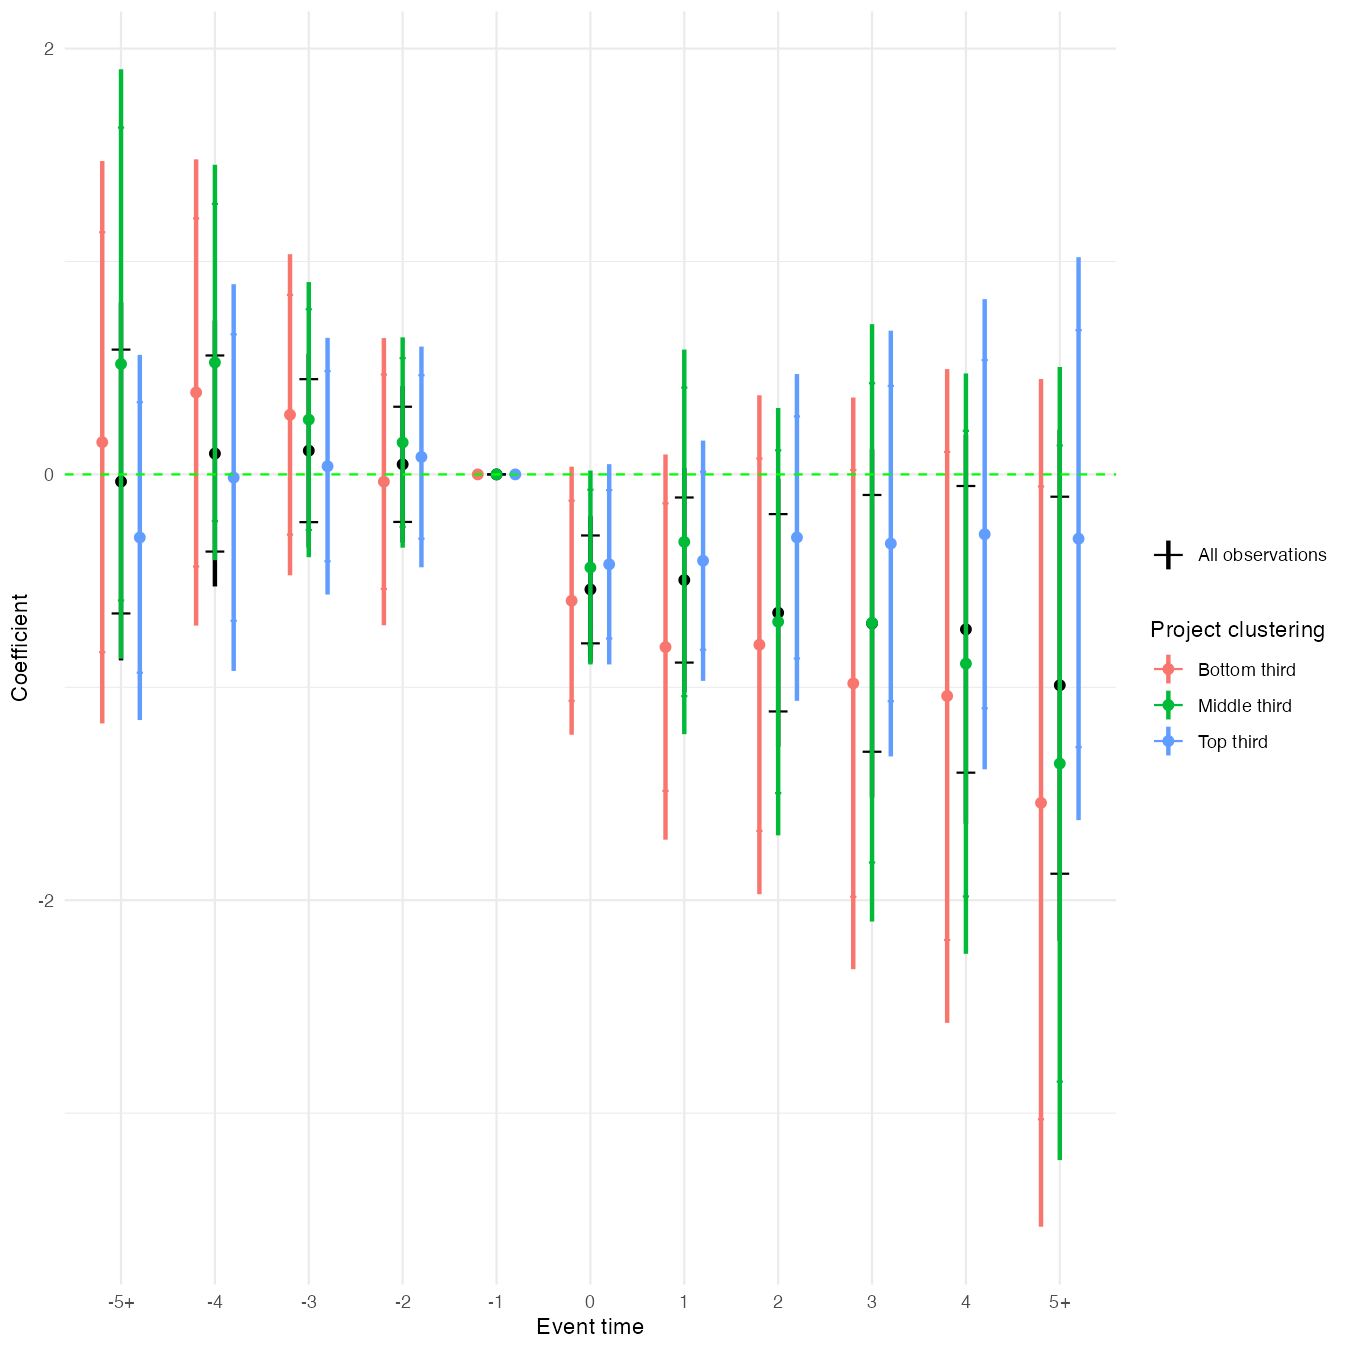
\includegraphics[width=\textwidth]{temp/project_clus_combined_2p_back_bin_third.png}
    \caption{PRs opened}
    \label{fig:clustering_outcome}
  \end{subfigure}\hfill
  \begin{subfigure}[b]{0.32\textwidth}
    \centering
    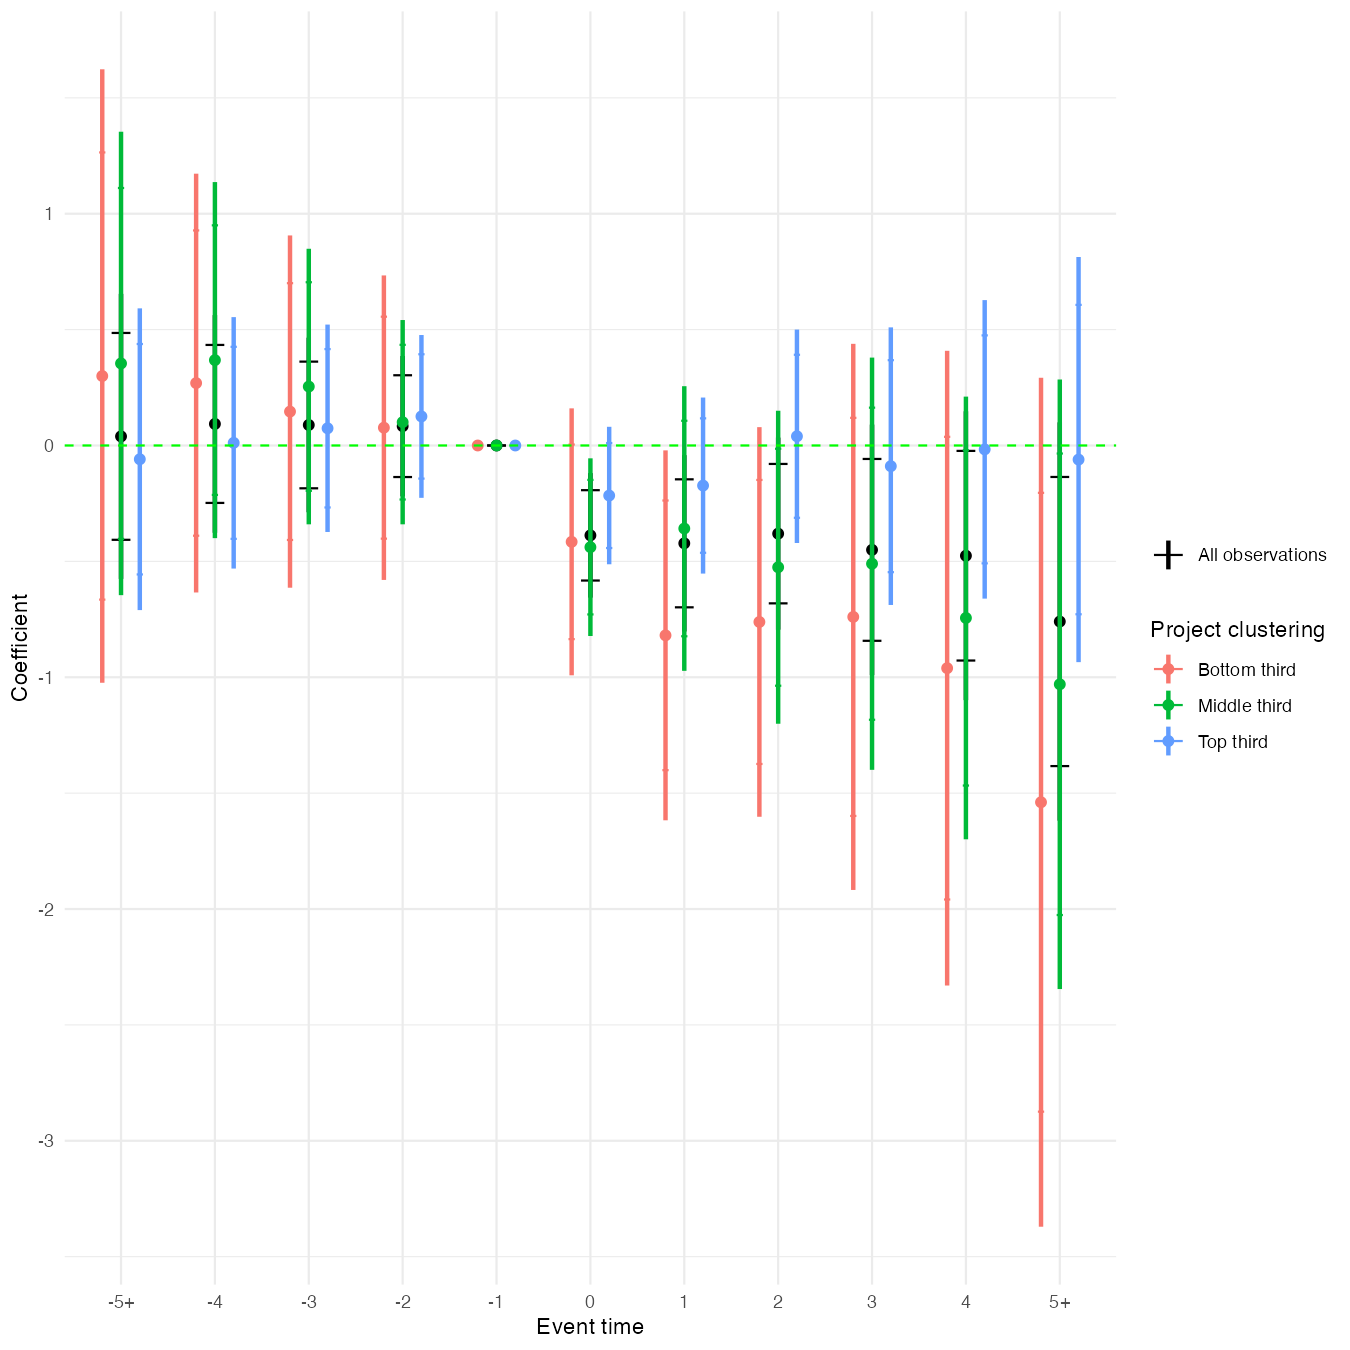
\includegraphics[width=\textwidth]{temp/project_clus_cc_combined_2p_back_bin_third.png}
    \caption{\# people opening PRs}
    \label{fig:clustering_cc}
  \end{subfigure}\hfill
  \begin{subfigure}[b]{0.32\textwidth}
    \centering
    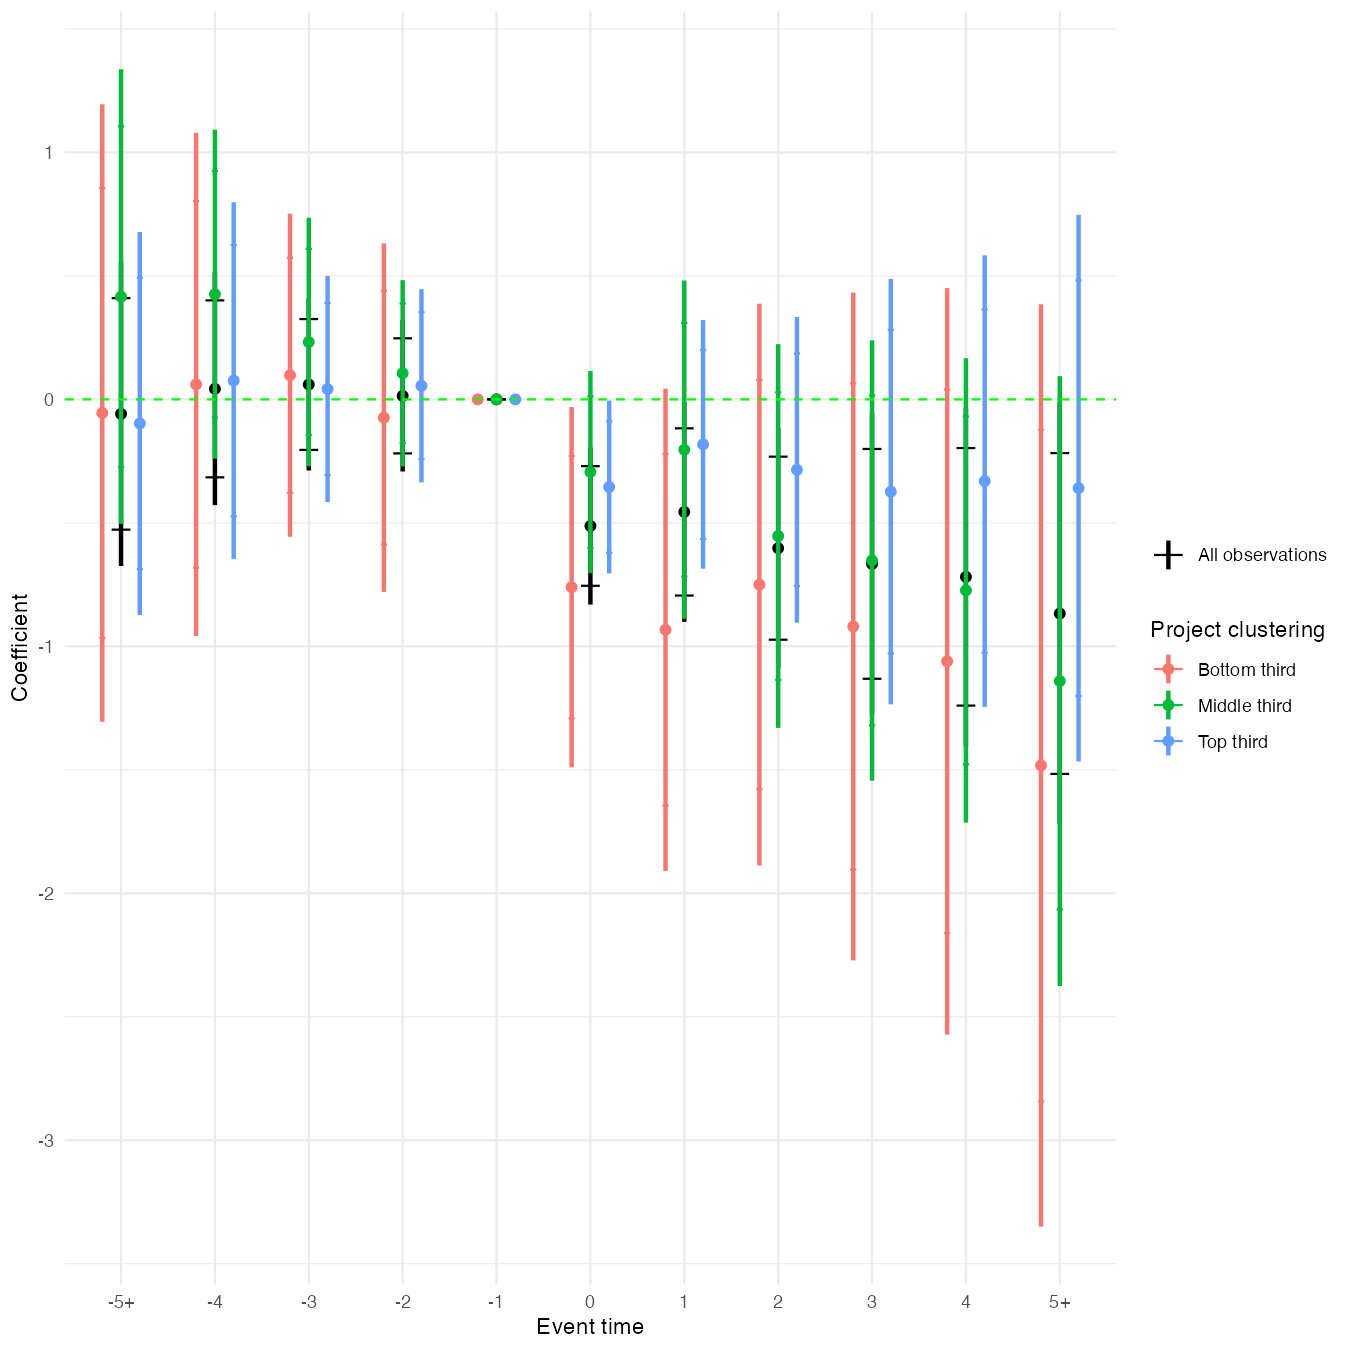
\includegraphics[width=\textwidth]{temp/project_clus_avg_combined_2p_back_bin_third.png}
    \caption{Avg.\ PRs opened pp}
    \label{fig:clustering_avg}
  \end{subfigure}
  \begin{subfigure}[b]{0.32\textwidth}
    \centering
    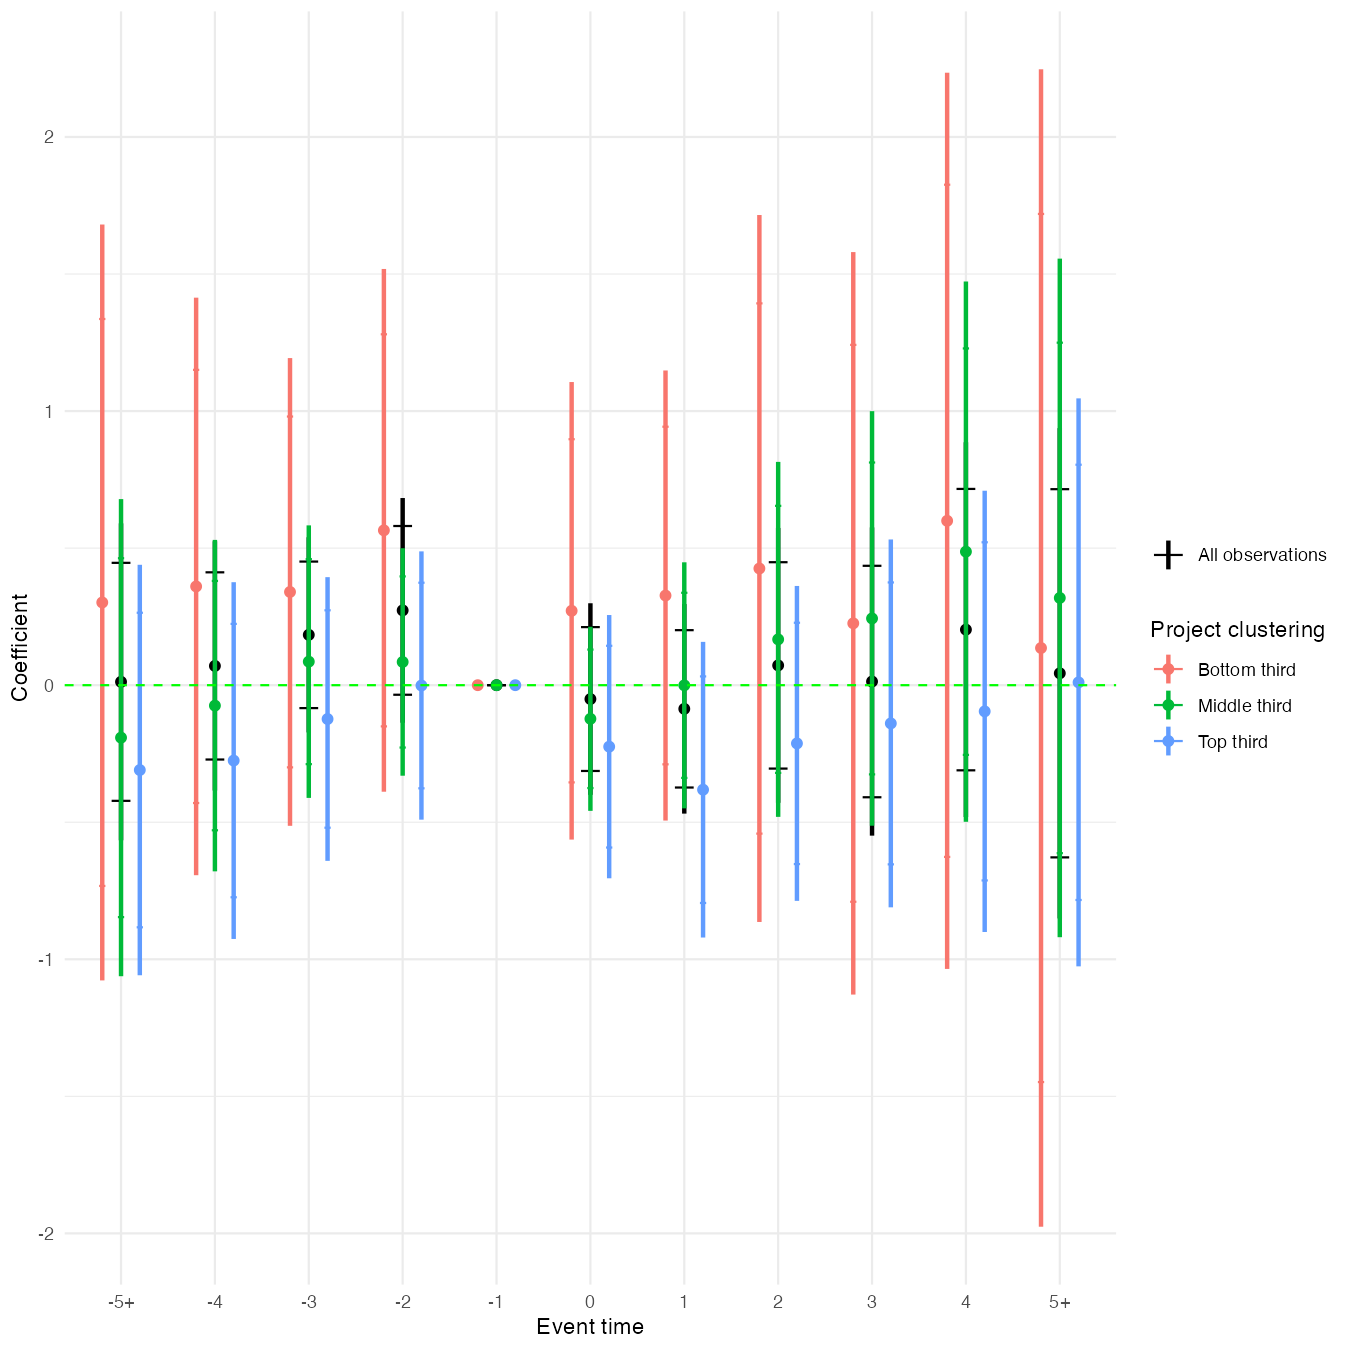
\includegraphics[width=\textwidth]{temp/project_clus_issues_combined_2p_back_bin_third.png}
    \caption{Issues opened}
    \label{fig:clustering_issue}
  \end{subfigure}
  \begin{subfigure}[b]{0.32\textwidth}
    \centering
    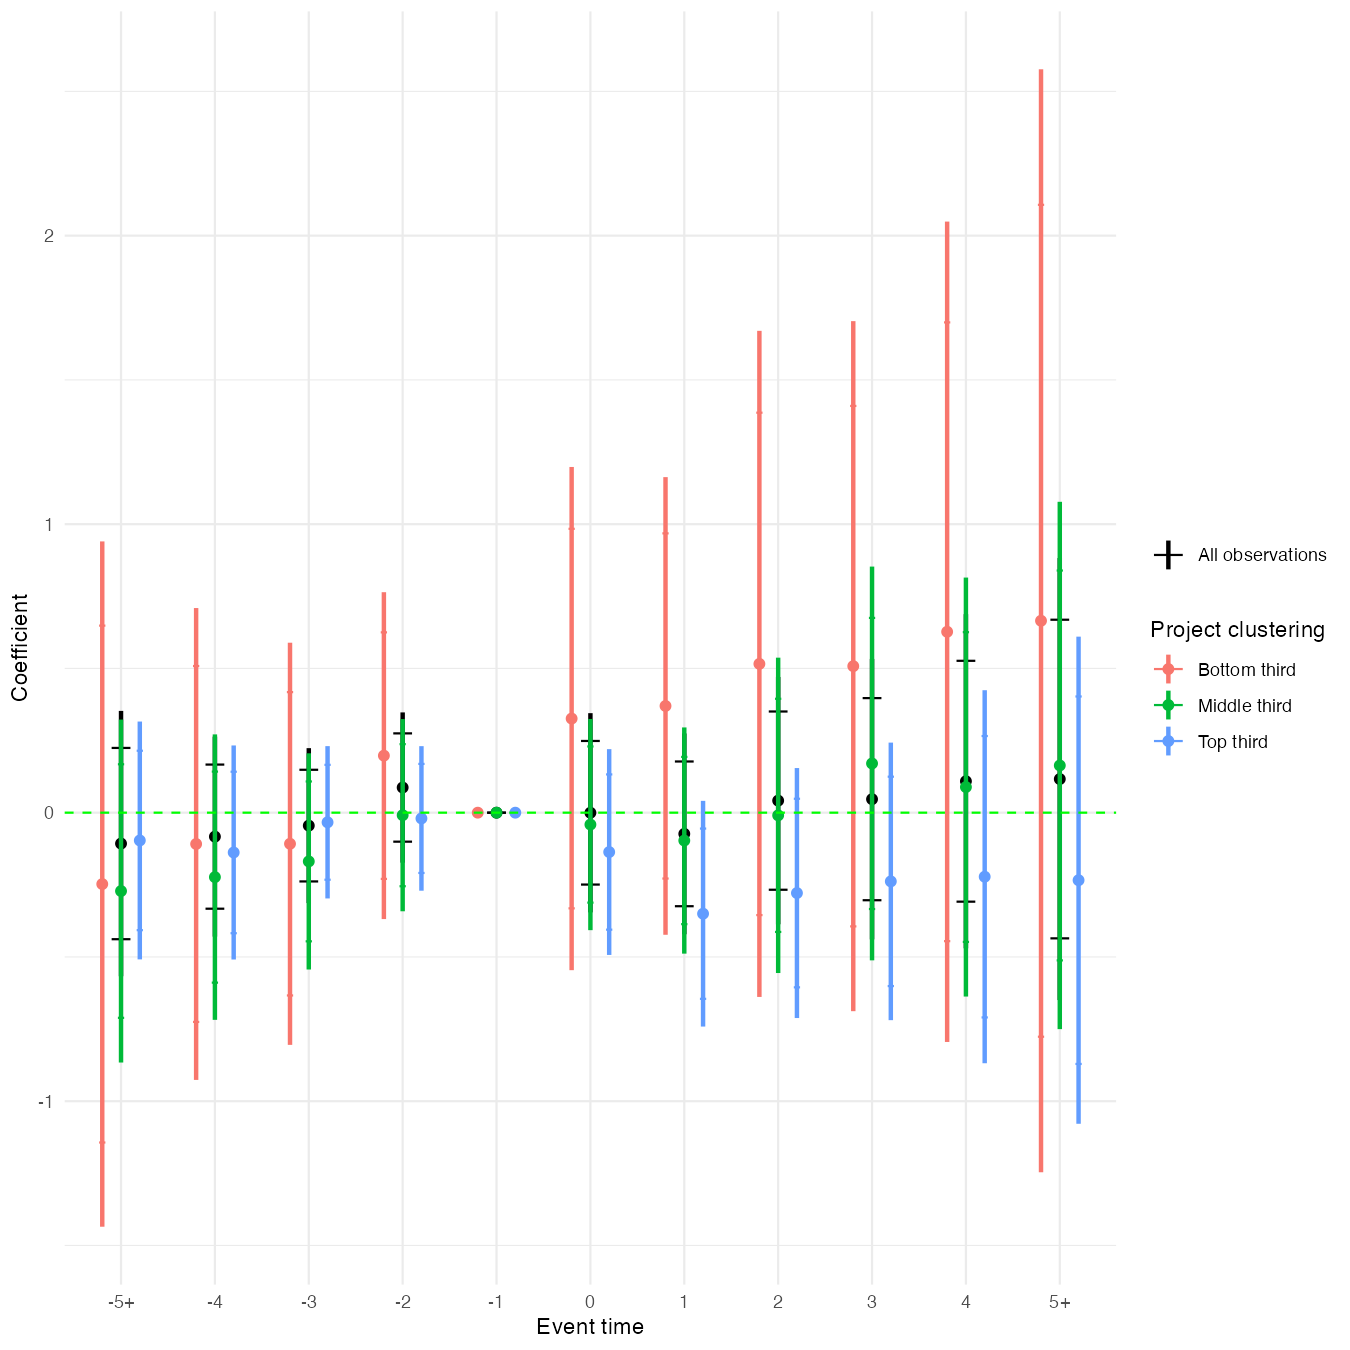
\includegraphics[width=\textwidth]{temp/project_clus_issues_cc_combined_2p_back_bin_third.png}
    \caption{\# of people opening issues}
    \label{fig:clustering_issue_cc}
  \end{subfigure}
  \begin{subfigure}[b]{0.32\textwidth}
    \centering
    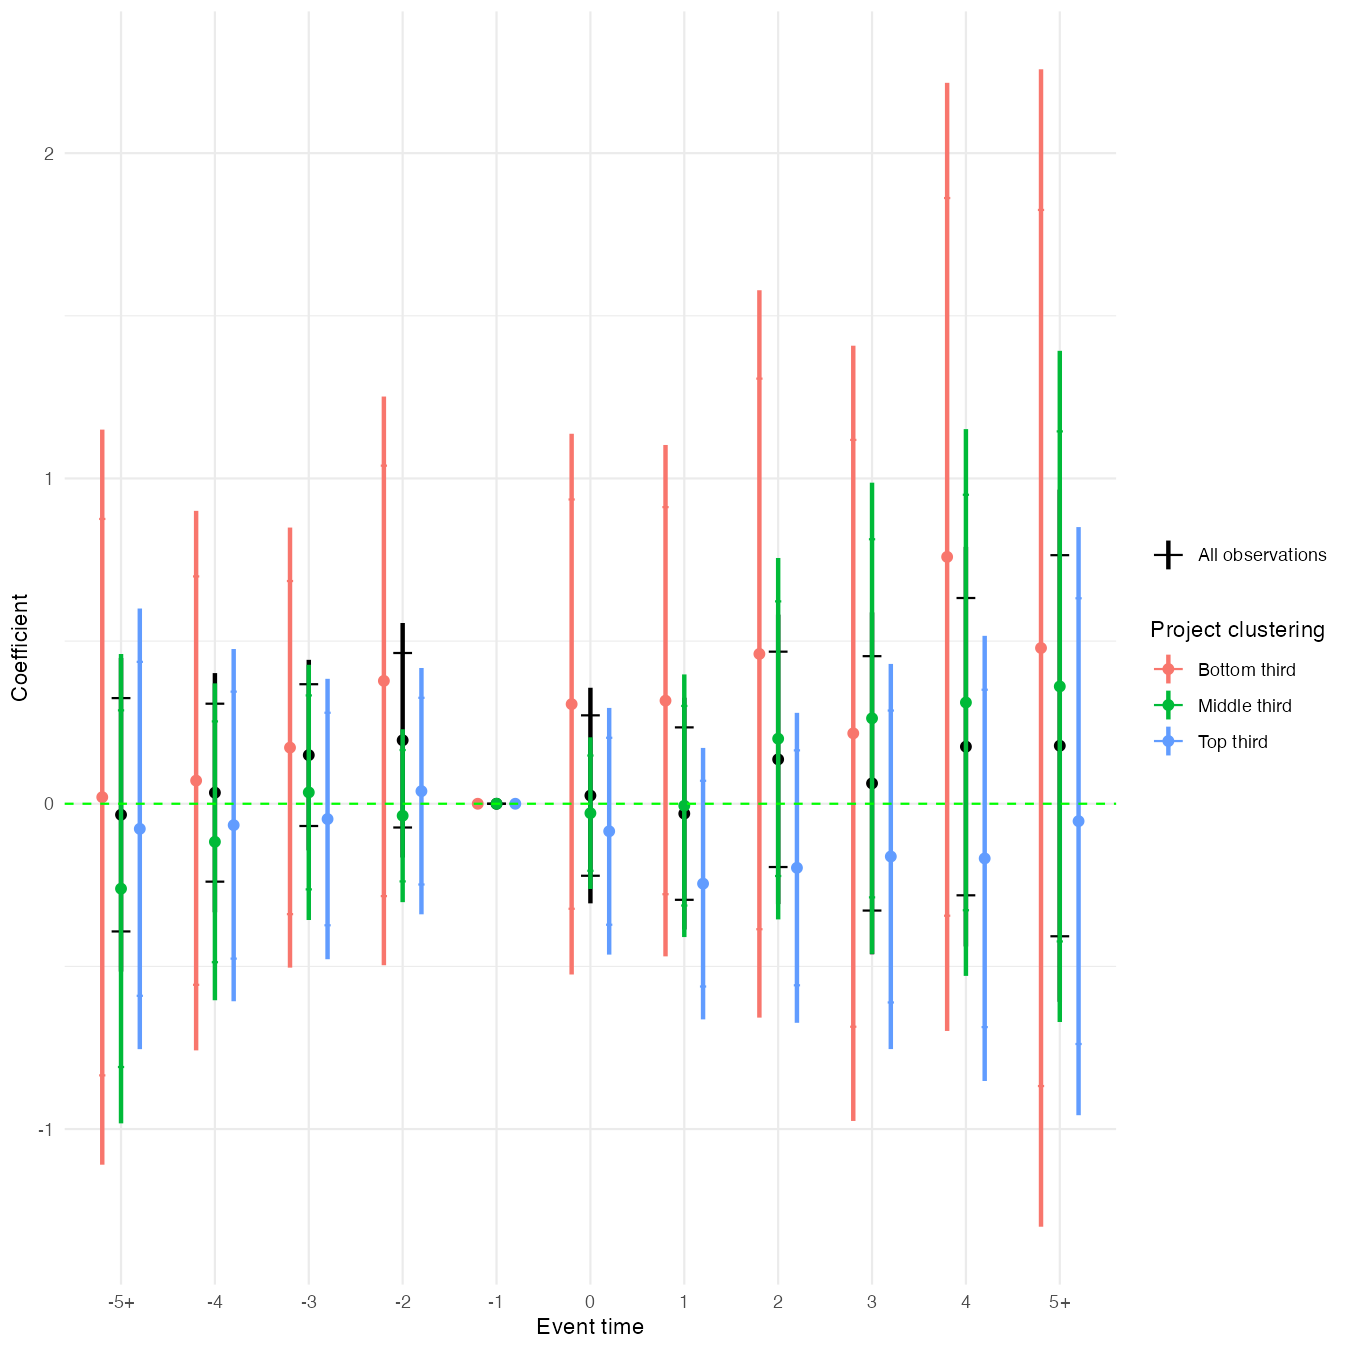
\includegraphics[width=\textwidth]{temp/project_clus_issues_avg_combined_2p_back_bin_third.png}
    \caption{Avg. issues opened pp}
    \label{fig:clustering_issue_cc}
  \end{subfigure}
  \caption{Impact of clustering on various outcomes.}
  \label{fig:clustering}
\end{figure}

    \todo[inline]{Add more controls for contributor importance, such as "authored commit share", "truckfactor status"}
    \item Recall that clustering is defined as the following: Across all key contributors, we compute the average share of each key contributor's collaborators who also work with other key contributors
    \item \textbf{Observations}
    \begin{enumerate}
        \item The effect gets worse over time, but doesn't vary in the beginning, as shown in Figure~\ref{fig:clustering_outcome}
        \item This isn't due to a change in the \# of issues opened. It seems like there aren't trends indicating decreased issues opened. If anything, clustered projects are most affected.
        \todo[inline]{SEE BELOW}
        \begin{enumerate}
            \item First, show that the rate of issue to PRs is actually decreasing in projects over time, and this happens more in projects that are less clustered
            \item Second, explore a variety of reasons for why unclustered projects are causing issues to not be converted. See below for an extensive list of reasons (broad ideas, have to think about specific details)
        \end{enumerate}
        \todo[inline]{Operationalization of step 1: Link issues to PRs either through the explicit linking, or by checking issue comments to see if they mention the PR. \\
        2. Calculate the rate\\
        3. Categorize people as issue opener, key contributor(s) and other discussants\\
        4. Proceed with the rest of the steps. \textbf{BEFORE STARTING BELOW, THINK ABOUT CONDENSING, REORDERING AND EXECUTION. }}
        \todo[inline]{For all of these think about variation by organizational structure, and the implications. Also, when evaluating effects, ask about the possibility of a mechanical effect. \\
        1. General data questions\\
        - Departed specific \\
        a) What \% of PRs were opened by the departed (just use open, not authored), and what \% of the last/last two non-author comments were made by the departed?  What \% of first replies are made by the departed (unconditional + conditional on a first reply existing)? How long does this take for the departed (and for all first repliers)\\
        \textcolor{white}{If the statistics vary, I would be concerned about mechanical effects. If these statistics don't vary, all is well. You can't use an event study with this, but the goal is to understand descriptively whether projects with different organizational structures differ}\\     
        - General\\
        a) # comments/issue, # ppl participating/issue, \% closed, attempted close (non-author responded), \textcolor{red}{Add more here - maybe some fo the response time work}\\
        \textcolor{white}{I'm hoping to better understand how issue discussion might have changed in response to departure and whether the effect varied by organizational structure. This will provide me with a better understanding of how organizational structure might be affecting issue discussion, and how changes in issue discussion lead to less PRs opened. It's possible that this may be too broad and I will need to find a way to connect this more specifically to departure. I can probably do event studies for this - think I already have event studies for \% closed}\\
        b) How often do issue openers also open a PR (in the same period, next two periods, etc)? What about if we split this statistic into "first-time" issue openers vs. non "first-time", or "important" vs. "unimportant". Also, think about ways I can better understand how joint participation across issues + PRs varies is affected by departure and varies by organizational structure \\
        \textcolor{white}{I'm hoping to better understand whose driving the effect in PRs. Understanding whether it's driven by experienced or fringe contributors can provide a clearer understanding of the effect of organizational structure, and also narrow down specific effects. For example, if it's fringe contributors who aren't opening PRs, I would want to better understand why and how they're receiving less support to open the PRs. If it's important contributors who aren't opening PRs, I would want to understand what knowledge they're missing now that the departed contributor is gone. }\\
        \textcolor{purple}{1) \% of PRs opened by departed: There are mechanical differences based on cluster that I should be concerned about. However, I'd expect the effect to be immediate if there was a mechanical effect?? } 
        c) How do the characteristics of opened PRs change? Such as 1) \% linked to an issue, 2) length of PR text, 3) \# of files changed, code changes, etc\\
        \textcolor{white}{I'm hoping this will provide further nuance about changes that are happening in projects that are more/less unclustered.}
        }
        \todo[inline]{Other planned todos
        1) Quantify relationship to the departed contributor (\textbf{work on below, tbd})
        1. were they connected to the departed contributor? How much did they interact? Across how many problems (issues + prs) and fields (issues, prs distinct) did they interact?\\
        2. Were they also connected to other departed contributors? How long did they stay? \textbf{opportunity to think further here - What's the effect of collaboration?}) \\
        ii) Analyze outcomes \textbf{work on below, tbd}\\
        2) Can I prove this is wrong: Effect driven by differences in wrapping up the departed's work? Doesn't seem so bc short-term but who knows?\\
        3) How do the characteristics of PR reviewing change (reply time, length, \# of people involved, \# of review comments, iterations of changes requested)
        4) Consider how https://docs.google.com/document/d/1nBp7vdNo48EcdtpVeklCczMOD8eH3-CKIkFl4PPBkvw/edit?tab=t.0 can be executed to provide further insights}
        \longterm[inline]{As I work, think about the different channels by which the departed contributor could impact overall quantity of PRs opened and the long-term story. Connect to themes such as "knowledge about project workings that's lost" or whether "teams are more productive than individuals (same people, less cooperation)"}
        \todo[inline]{Aside: If I only use interactixons between clusters for issues, does that enhance the effects?}
        \item Activity decline is driven by both declines in participation (Figure~\ref{fig:clustering_cc}) and average activity (Figure~\ref{fig:clustering_avg}). How might each be related to organizational structure? \textbf{Working on explanations above}

        
        \todo[inline]{more advanced questions below}
        \item Are contributors in unclustered projects less substitutable, and contributors in more clustered projects more substitutable (which is why there is cooperation)?
        \item How do newcomers fit into organizations depending on clustering?

    \end{enumerate}

    \item There seems to be some interesting nuance here. At the project-level, too much imp<->imp communication is what dooms it. When it comes to imp<->imp what you don't want is to have had no communication with the departed. It also seems like too much communication doesn't help either.  
\begin{figure}[hp]
  \centering
  \begin{subfigure}[b]{0.48\textwidth}
    \centering
    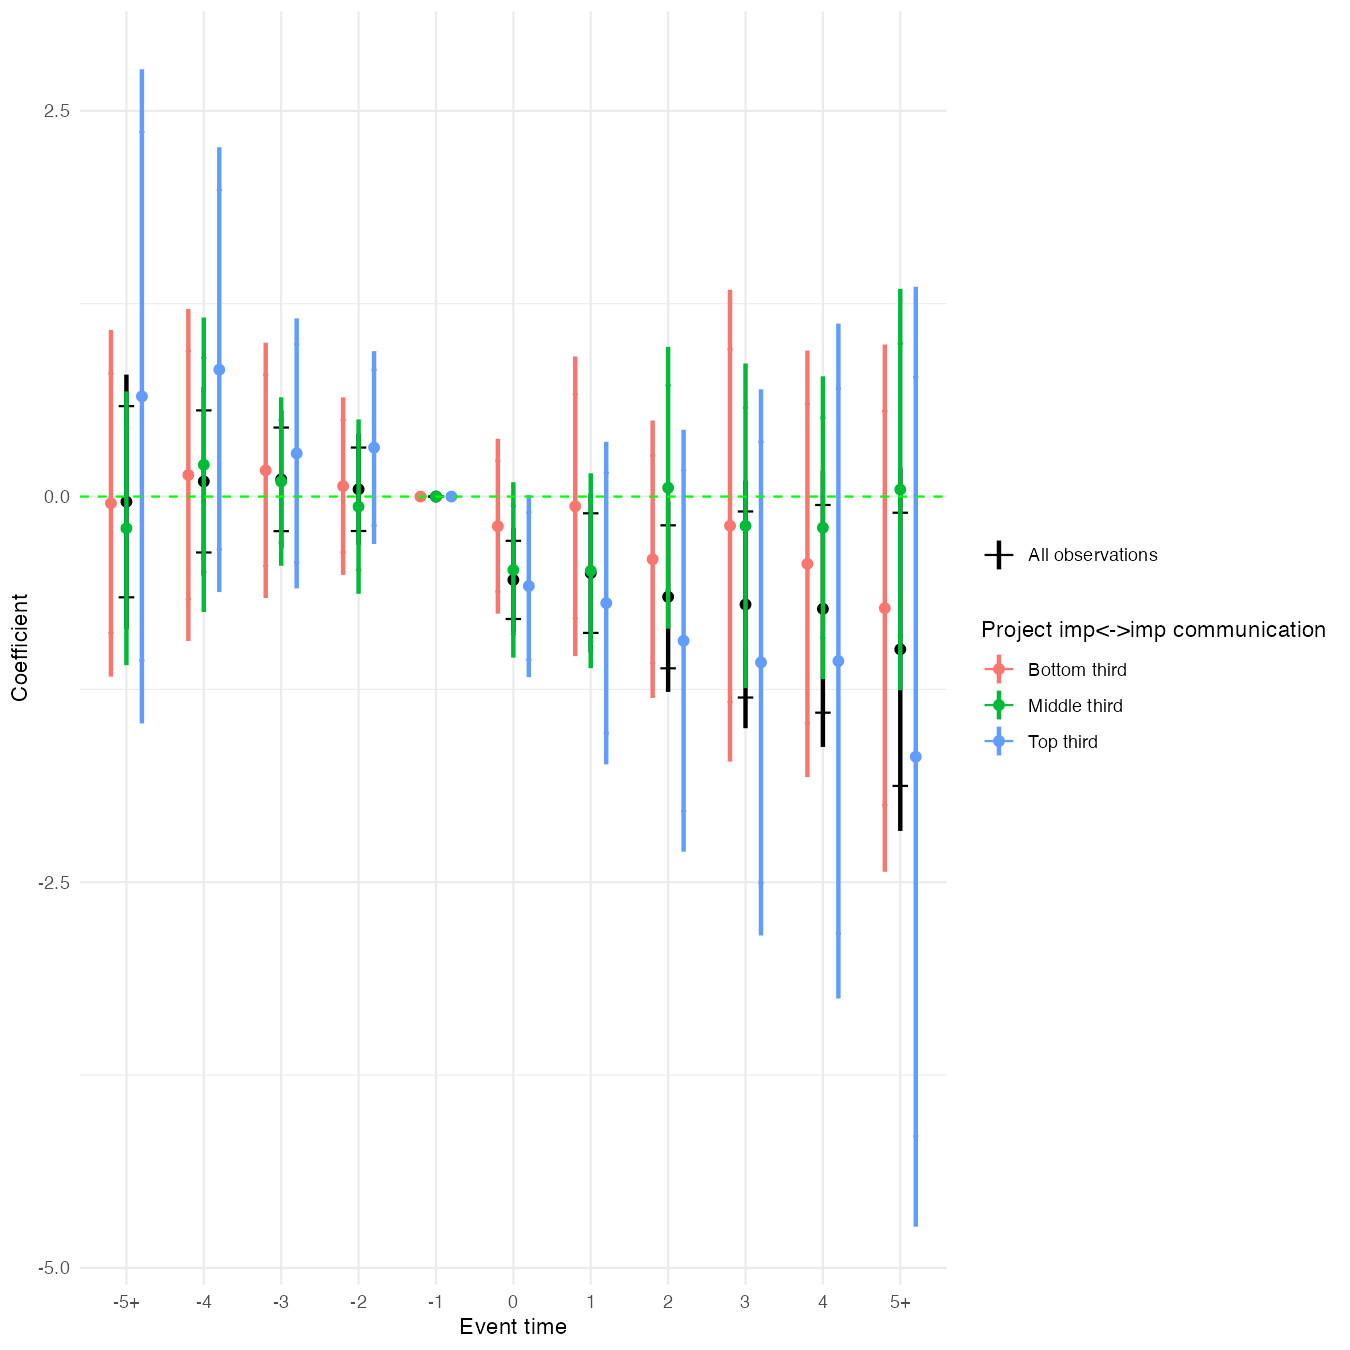
\includegraphics[width=\textwidth]{temp/imp_imp_combined_2p_back_bin_third.png}
    \caption{Imp<->Imp (project-wide)}
  \end{subfigure}
  \hfill
  \begin{subfigure}[b]{0.48\textwidth}
    \centering
    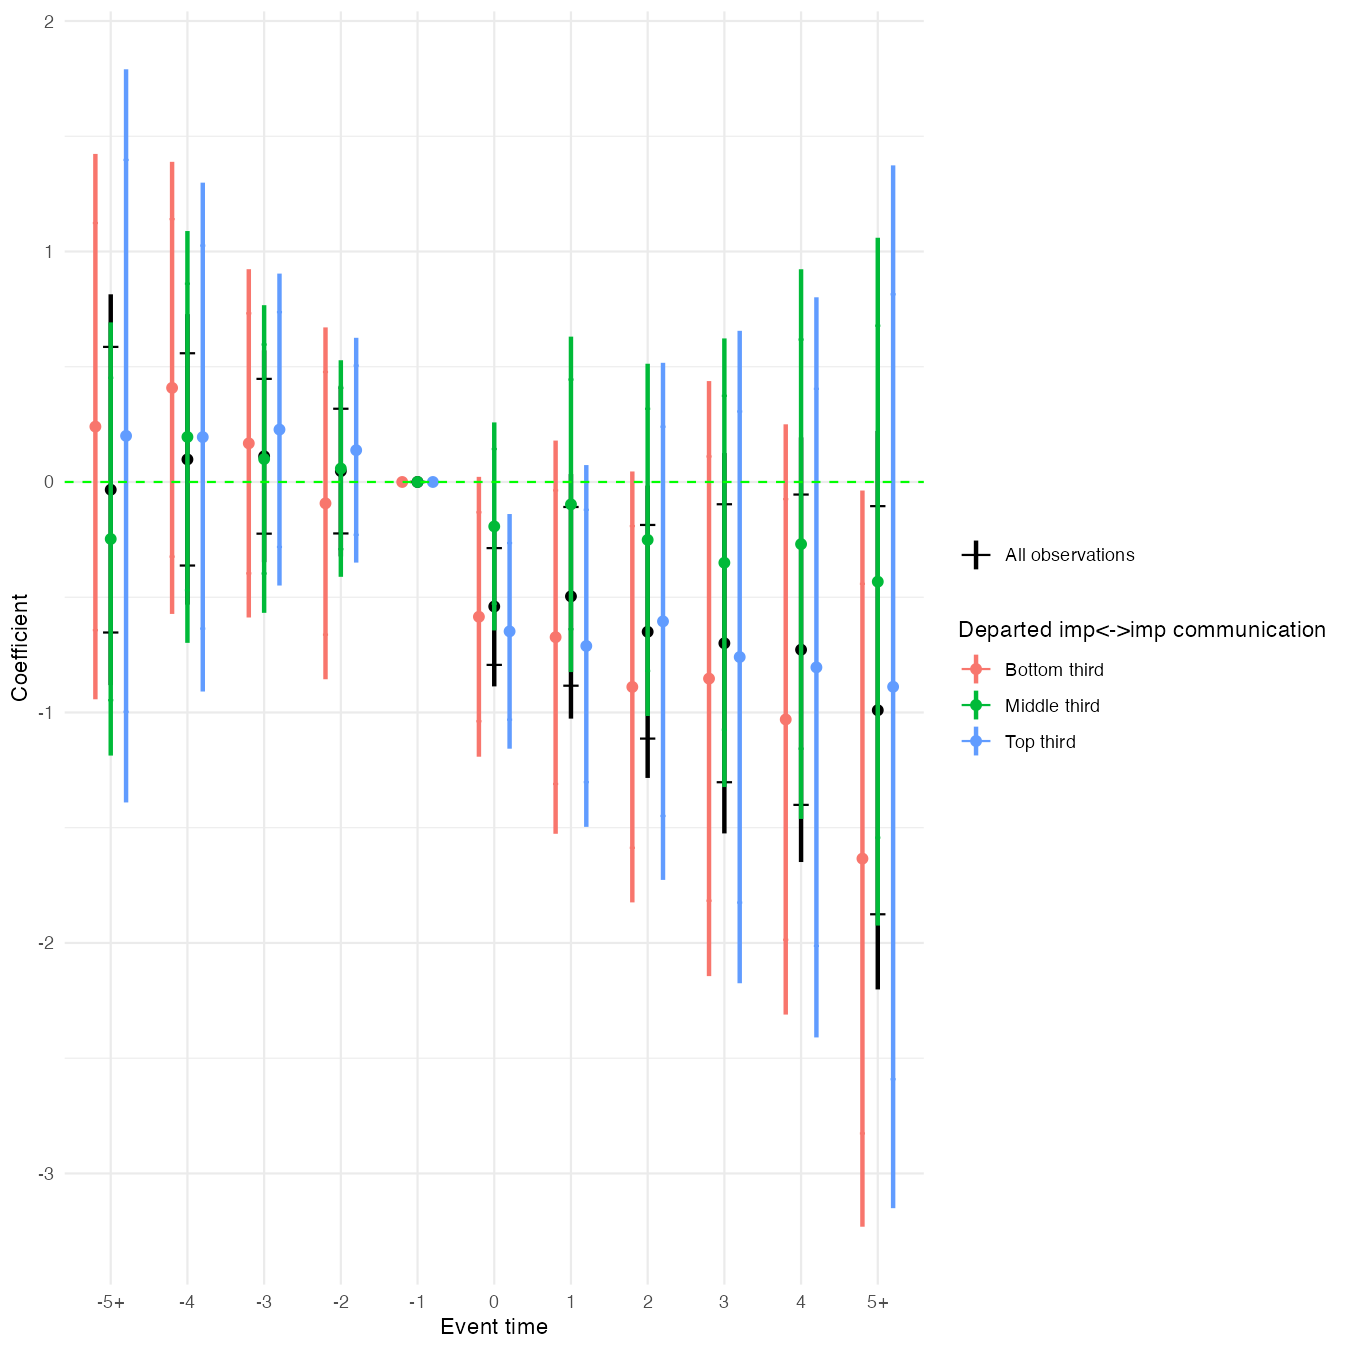
\includegraphics[width=\textwidth]{temp/imp_imp_dept_combined_2p_back_bin_third.png}
    \caption{Imp<->Imp (departed)}
  \end{subfigure}
  \caption{Impact of imp<->imp communication on post-departure outcomes}
\end{figure}
    \item Seems like middle amounts of imp<->other communication in the project are best (similar to imp<->other). For the departed, what's interesting is that 
\begin{figure}[hp]
  \centering
  \begin{subfigure}[b]{0.48\textwidth}
    \centering
    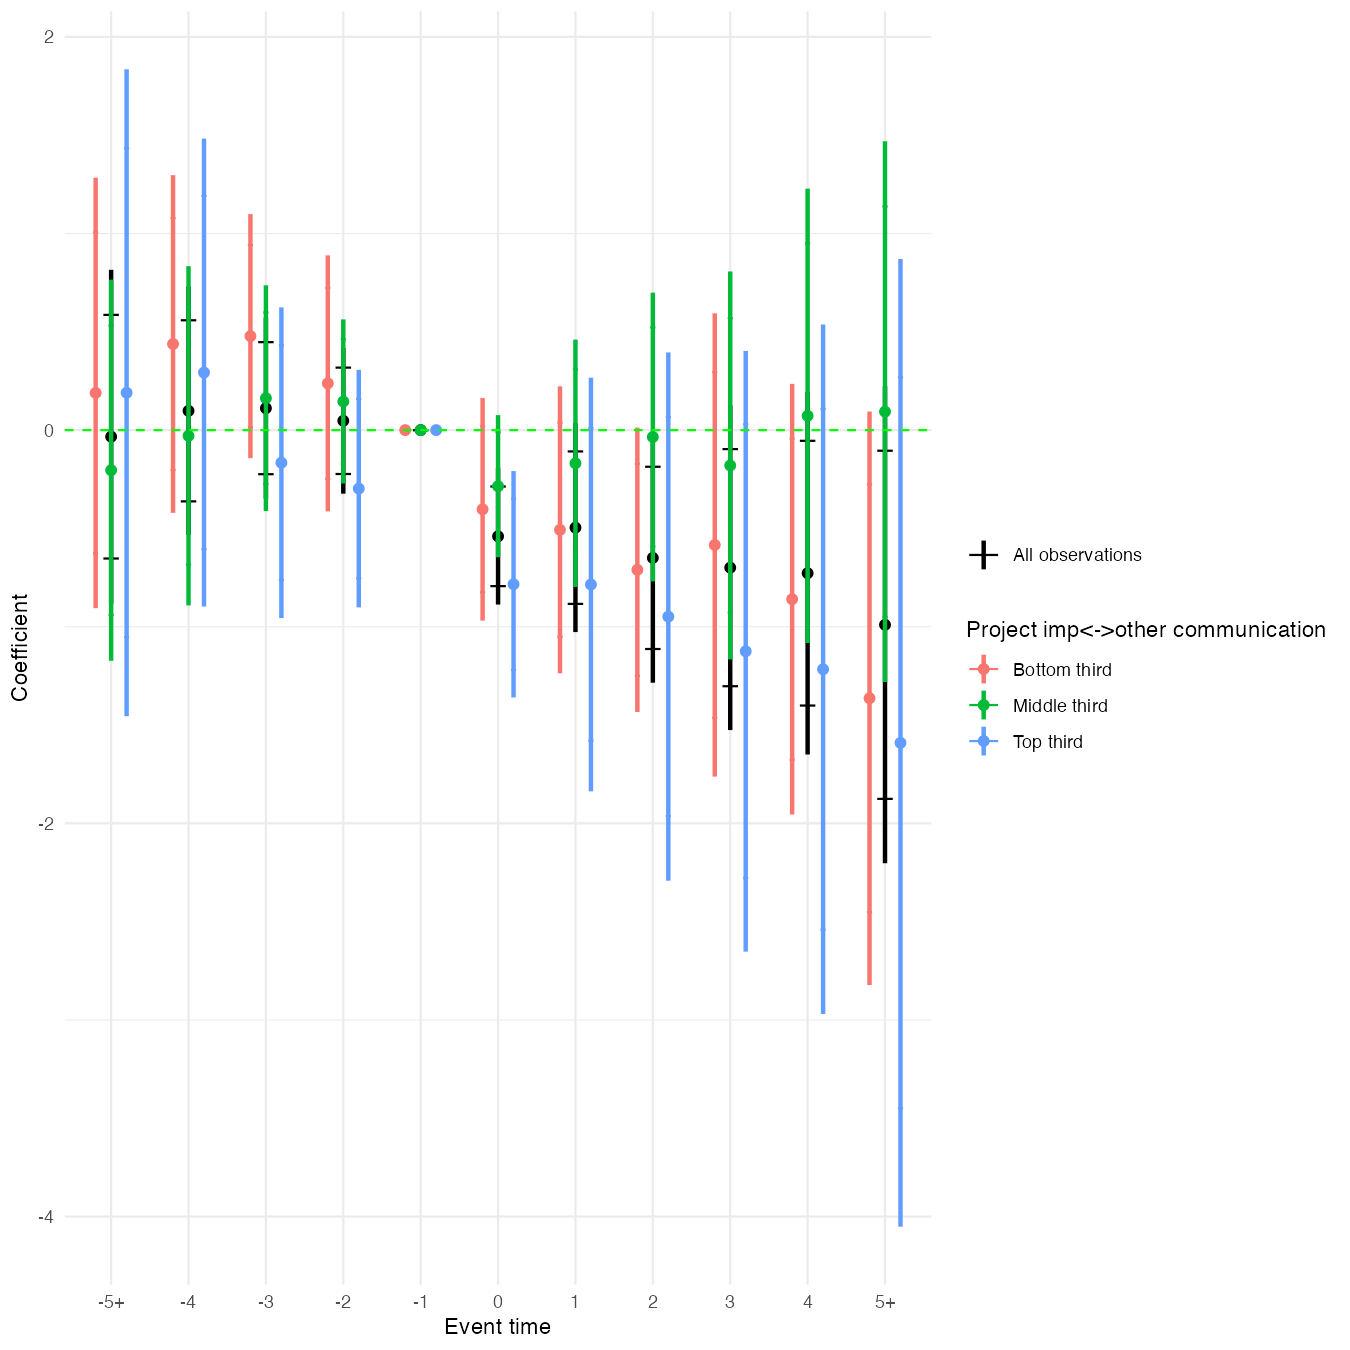
\includegraphics[width=\textwidth]{temp/imp_other_combined_2p_back_bin_third.png}
    \caption{Imp<->Imp (project-wide)}
  \end{subfigure}
  \hfill
  \begin{subfigure}[b]{0.48\textwidth}
    \centering
    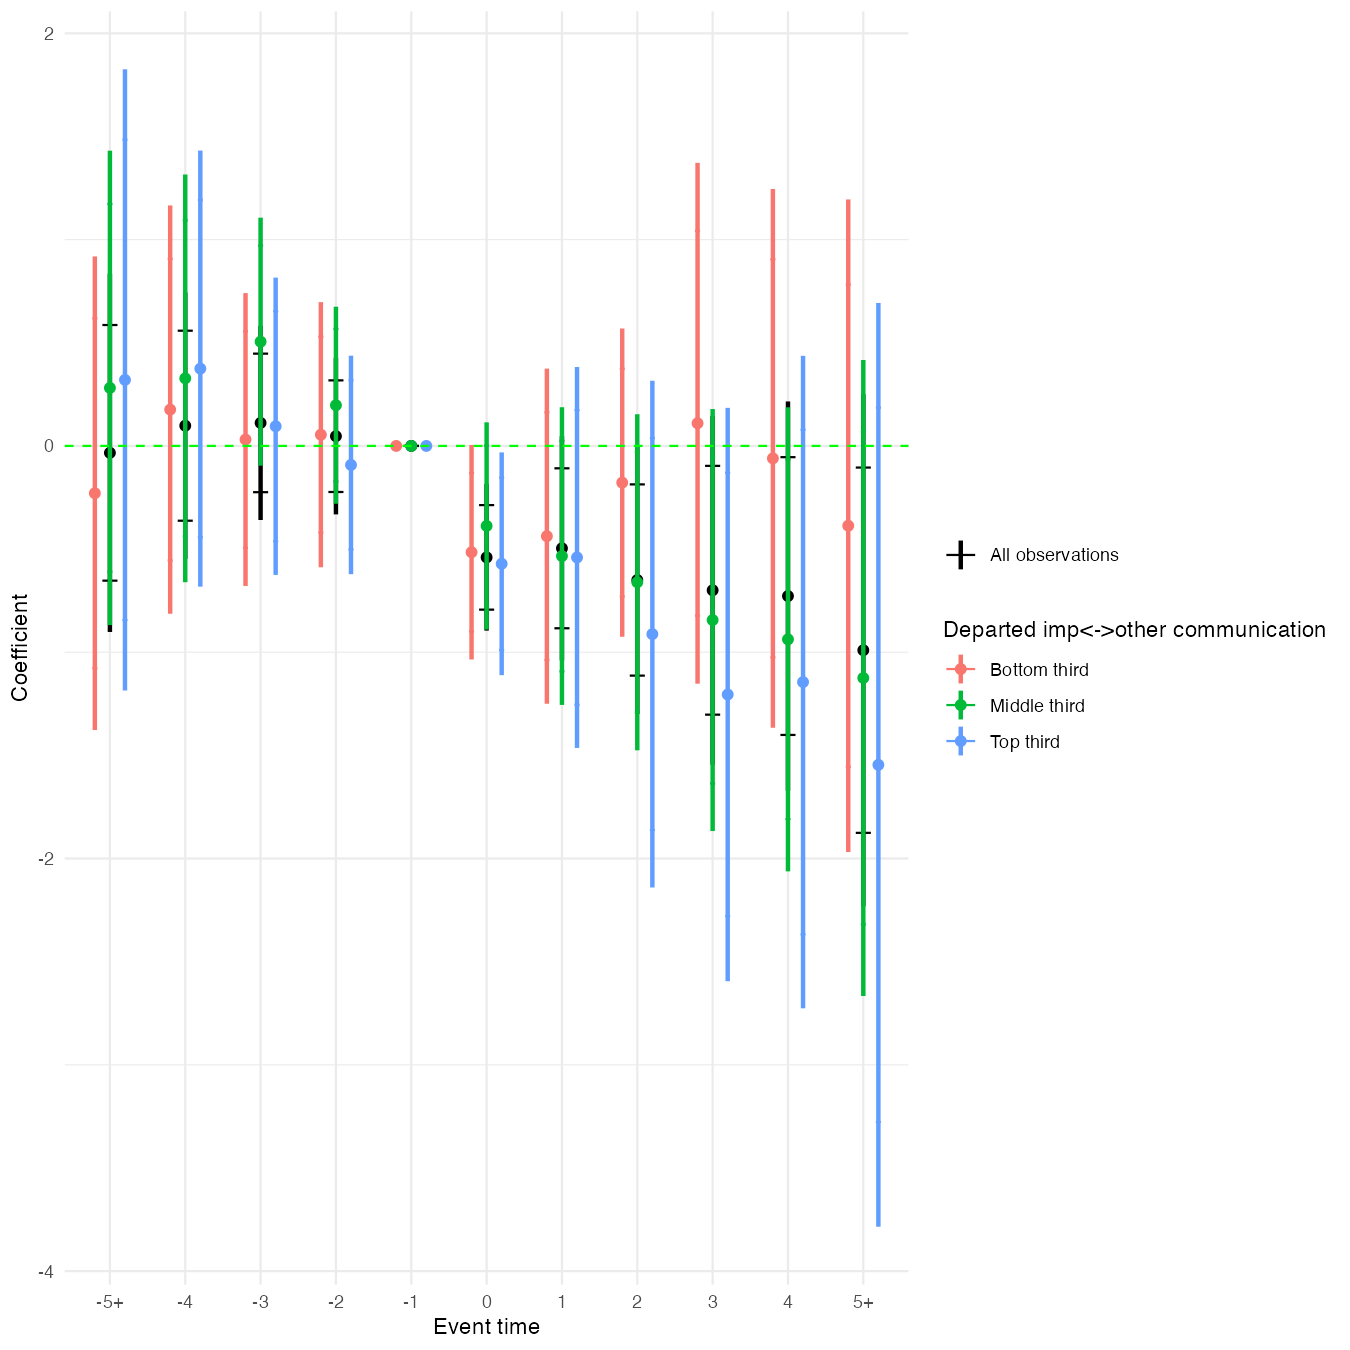
\includegraphics[width=\textwidth]{temp/imp_other_dept_combined_2p_back_bin_third.png}
    \caption{Imp<->Imp (departed)}
  \end{subfigure}
  \caption{Impact of imp<->imp communication on post-departure outcomes}
\end{figure}

\end{itemize}




- Departed contributor overlap doesn't seem to matter very much, but it seems like something that'd be good to look into robustness
- Communication the story is much more nuanced. Overall imp<->other communication, middle third is best. departed imp<->other communication, little is best in the long term?
- Overall imp<->imp communication: not that much is good, 




\section{Conclusion} \label{sec:conclusion}



\singlespacing


\clearpage

\onehalfspacing

\section*{Tables} \label{sec:tab}
\addcontentsline{toc}{section}{Tables}



\clearpage

\section*{Figures} \label{sec:fig}
\addcontentsline{toc}{section}{Figures}

%\begin{figure}[hp]
%  \centering
%  \includegraphics[width=.6\textwidth]{../fig/placeholder.pdf}
%  \caption{Placeholder}
%  \label{fig:placeholder}
%\end{figure}




\clearpage

\section*{Appendix A. Placeholder} \label{sec:appendixa}
\addcontentsline{toc}{section}{Appendix A}


\end{document}